\documentclass[dvipdfmx]{jsarticle}

\usepackage[utf8]{inputenc}
\usepackage[dvipdfmx]{graphicx}
\usepackage{float}
\usepackage{amsmath}

\begin{document}
    \title{情報通信工学 Assignment5}
    \author{電気電子工学科 03-180500 \\ 平井雄太}
    \date{2018年11月7日}
    \maketitle
    \section{}
    \subsection{}
    \begin{figure}[H]
        \centering
        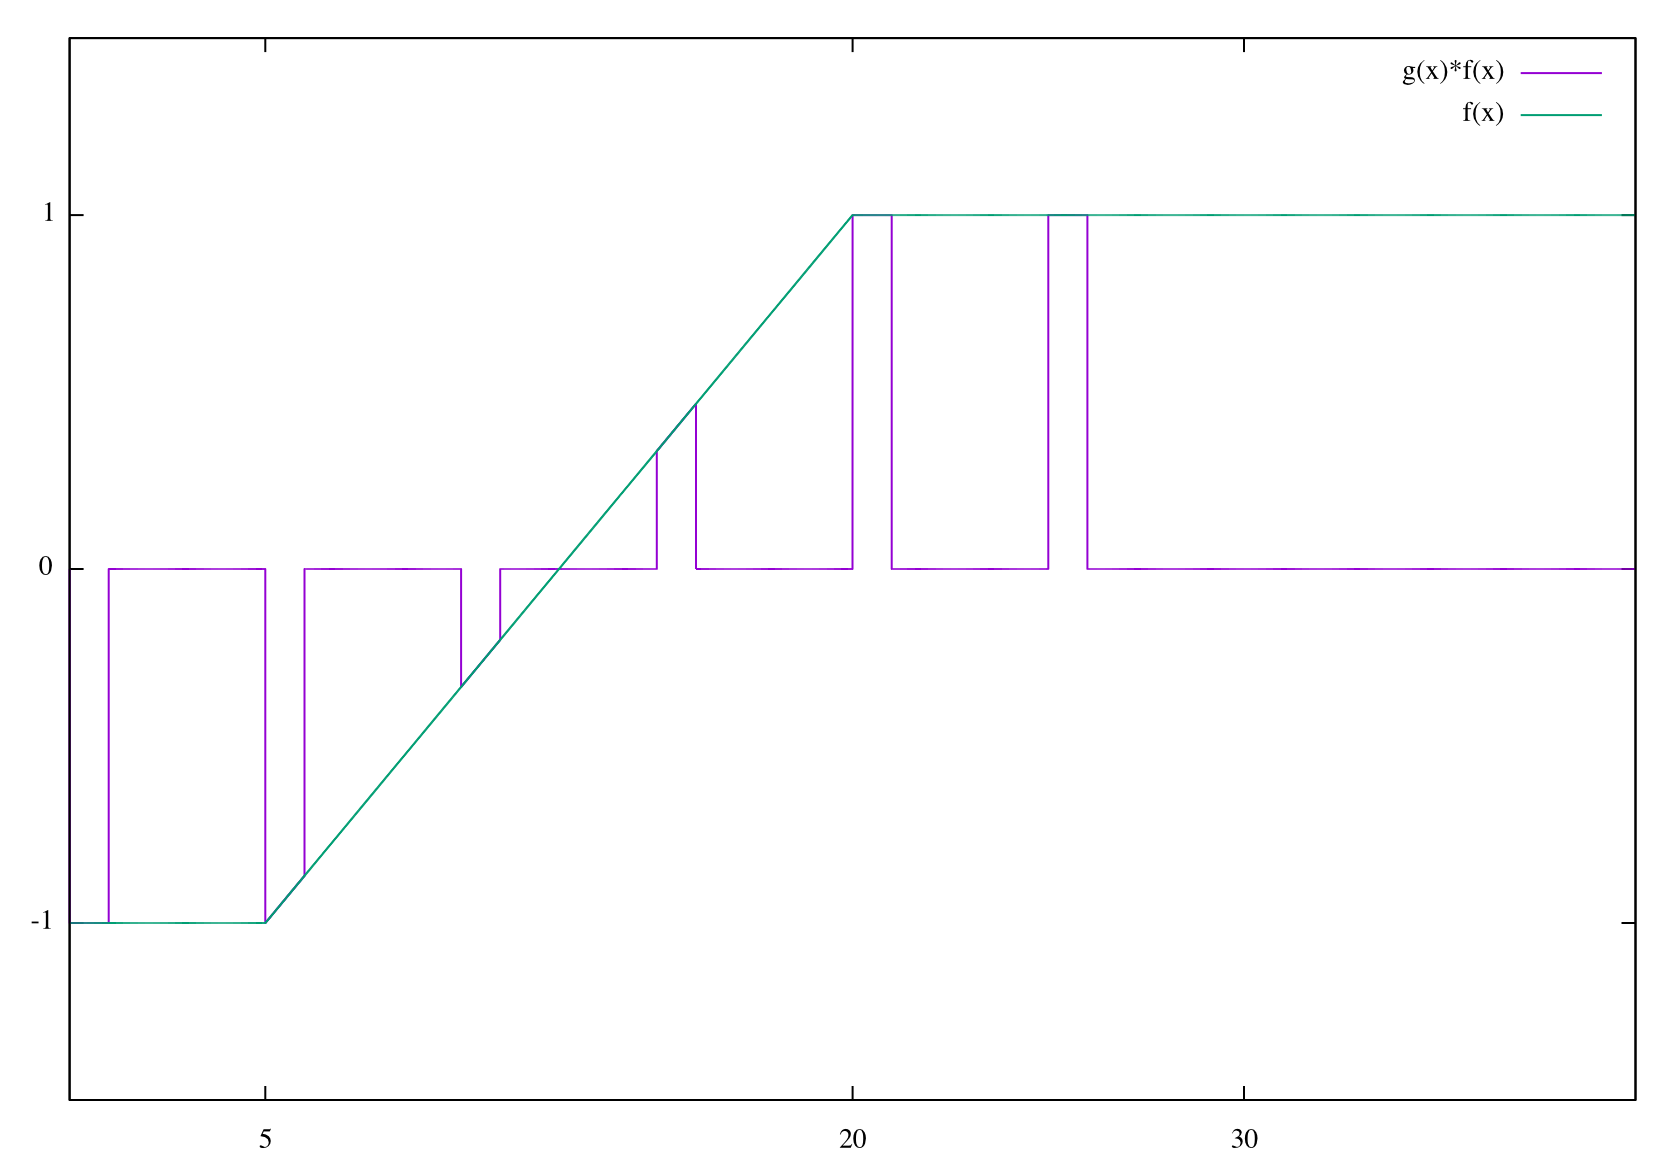
\includegraphics[width=10cm]{graph1.png}
        \caption{PAM波形}
        \label{fig:1}
    \end{figure}
    PAM波形を求めるには,パルス幅1ms, 200Hzの波と信号を掛け合わせればいい。
    よって図\ref{fig:1}のようになる。
    \subsection{}
    \begin{figure}[H]
        \begin{tabular}{cc}
            \begin{minipage}{0.45\hsize}
                \centering
                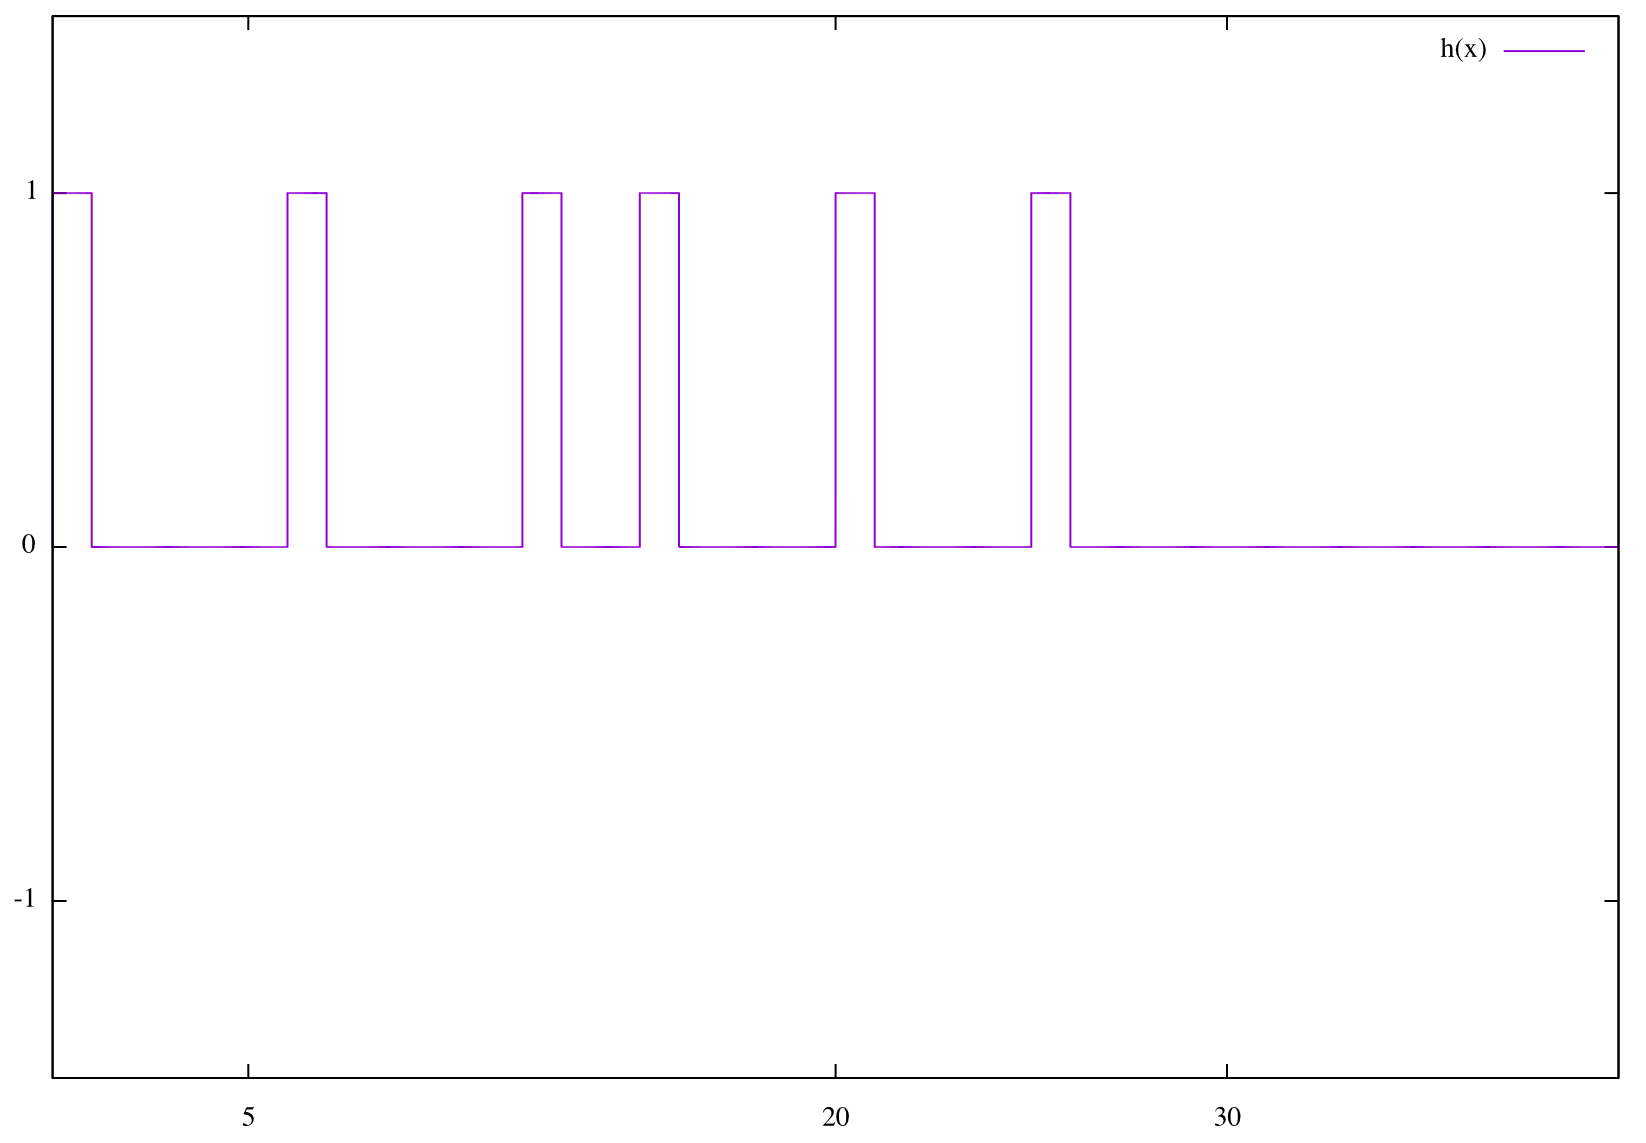
\includegraphics[width=0.9\hsize]{graph2.png}
                \caption{PPM波形の搬送波}
                \label{figure:2}
            \end{minipage} &
            \begin{minipage}{0.45\hsize}
                \centering
                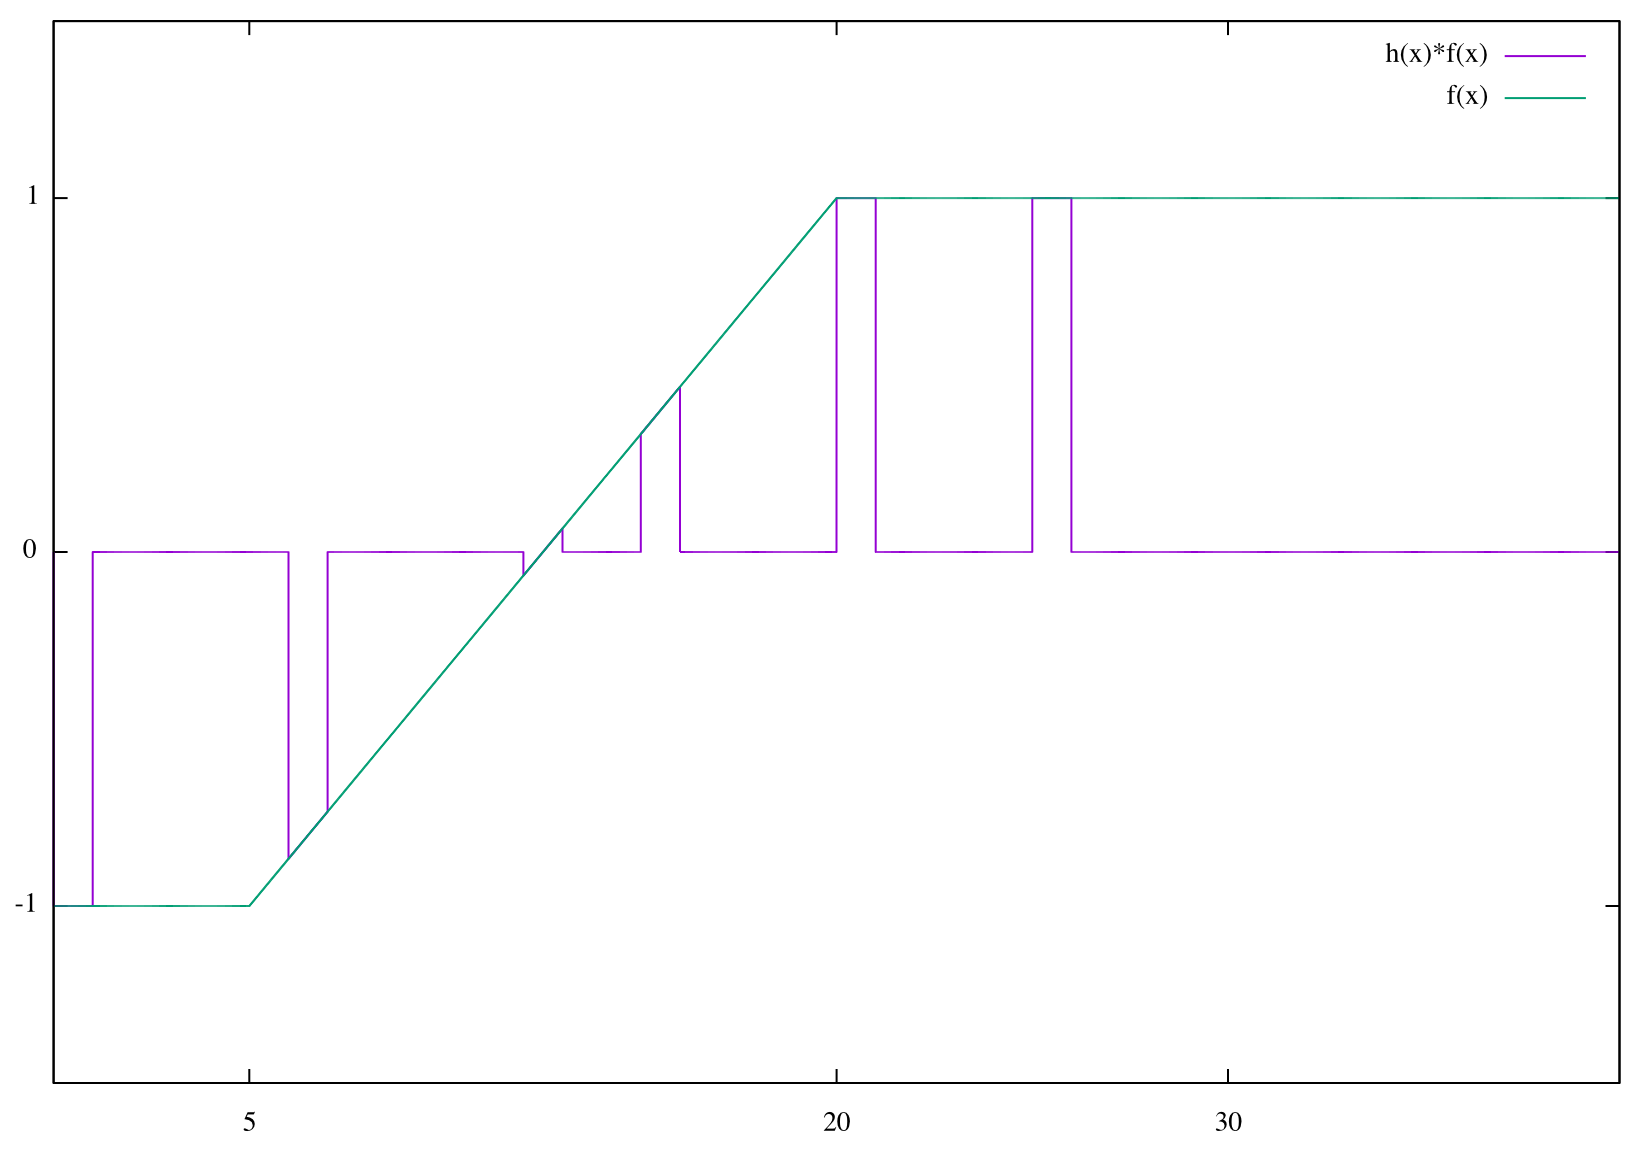
\includegraphics[width=0.9\hsize]{graph3.png}
                \caption{PPM波形}
                \label{figure:3}
            \end{minipage}
        \end{tabular}
    \end{figure}
    本文では搬送波について特に指定がなかったので、図\ref{figure:2}のような搬送波を想定した。
    この時のPPM波形は図\ref{figure:3}ようになる。
    \subsection{}
    \begin{figure}[H]
        \begin{tabular}{cc}
            \begin{minipage}{0.45\hsize}
                \centering
                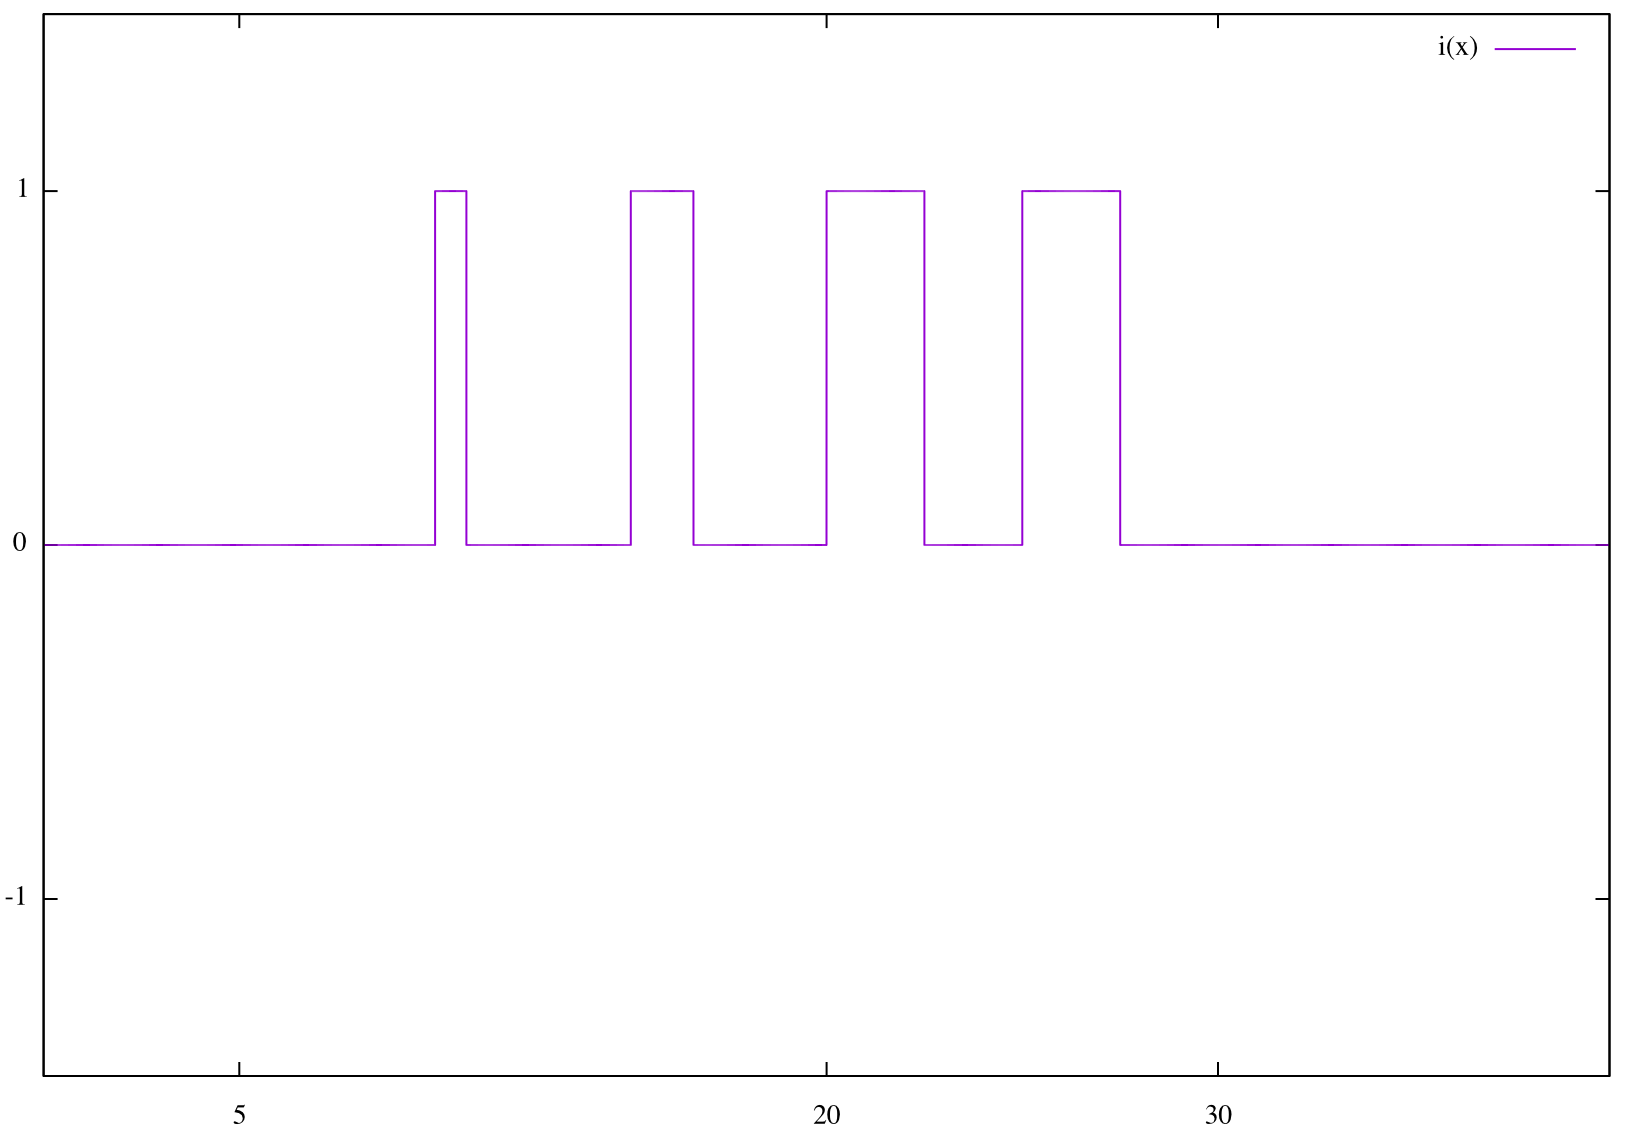
\includegraphics[width=0.9\hsize]{graph4.png}
                \caption{PWMの搬送波}
                \label{figure:4}
            \end{minipage} & 
            \begin{minipage}{0.45\hsize}
                \centering
                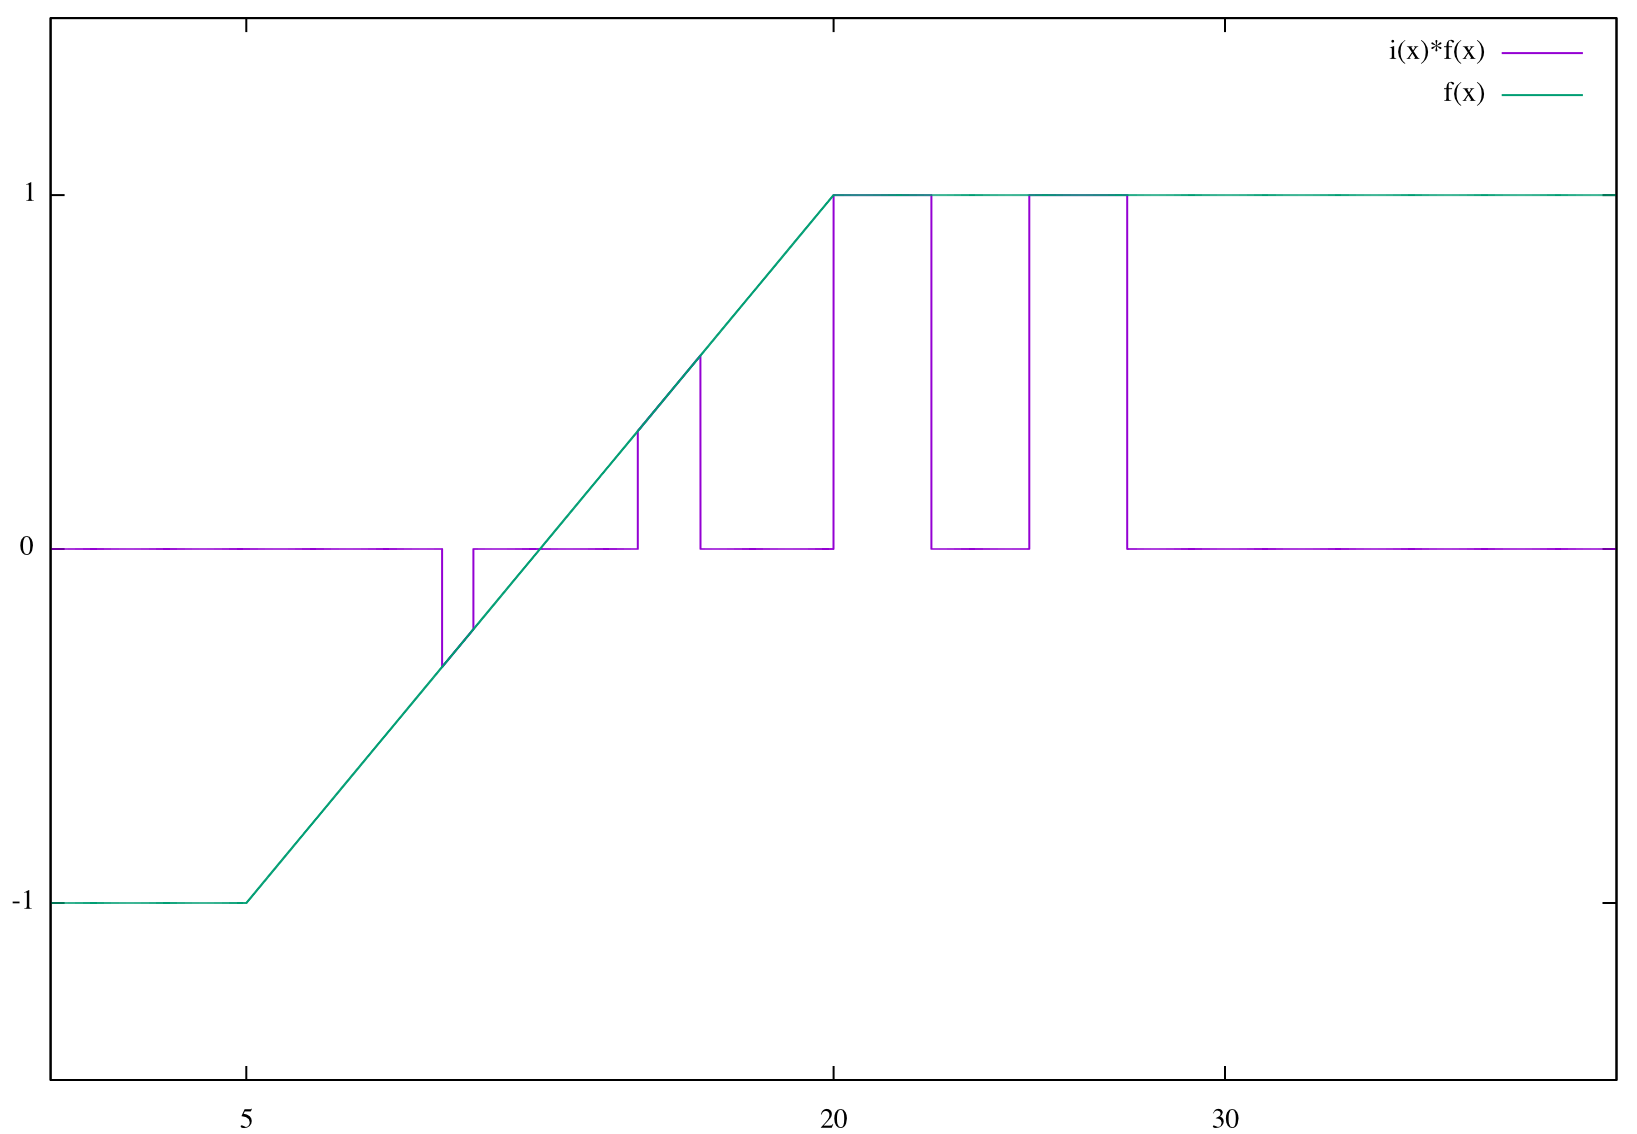
\includegraphics[width=0.9\hsize]{graph5.png}
                \caption{PWM波形}
                \label{figure:5}
            \end{minipage}
        \end{tabular}
    \end{figure}
    PWMでは、搬送波は信号の振幅に比例して幅が変われば良い。ここでは、$t = 5n[ms]$の時の
    振幅を$A(t)$として、幅が$\frac{1}{4}(A(t)+1)ms$となるように設定した。
    この時の搬送波を図\ref{figure:4}に、PWM波形を図\ref{figure:5}に示す。

    \subsection{}
    \begin{figure}[H]
        \centering
        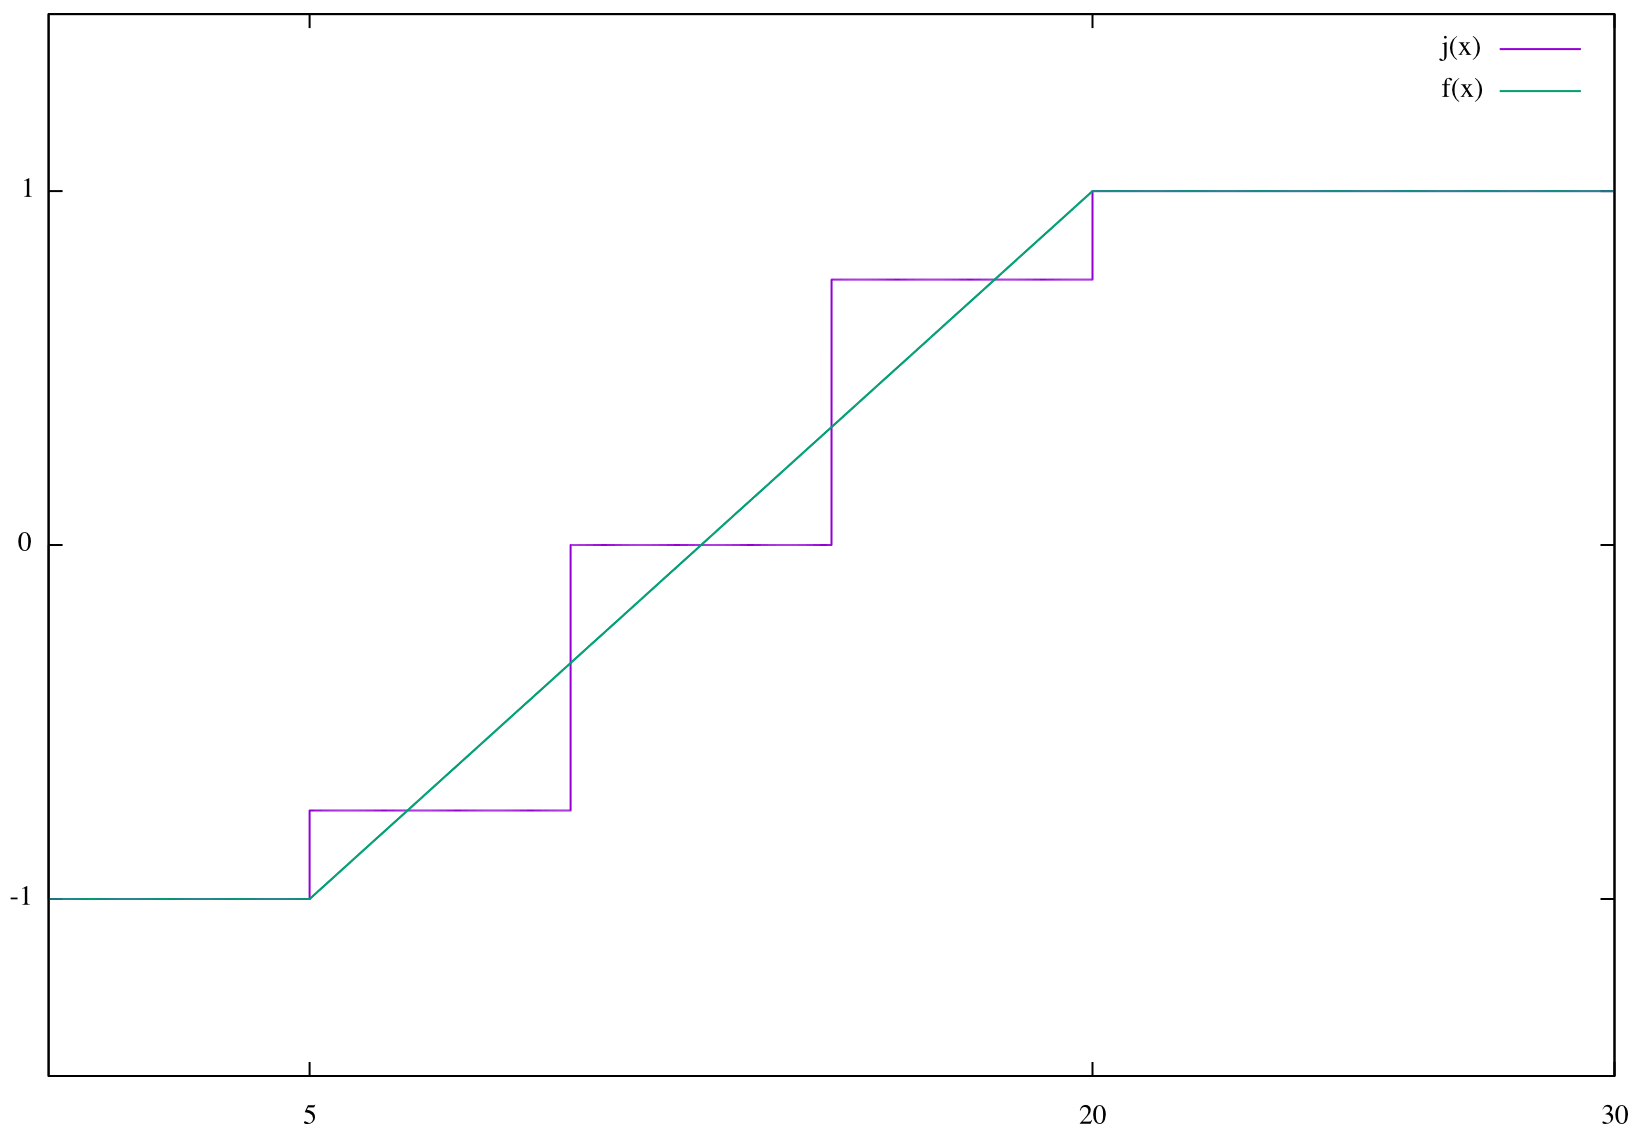
\includegraphics[width=0.7\hsize]{graph6.png}
        \caption{量子化された信号}
        \label{figure:6}
    \end{figure}
    \begin{table}[H]
        \centering
        \caption{各標本値の量子化誤差}
        \label{table:1}
        \begin{tabular}{c|ccc}
            サンプリング範囲[ms]&信号の振幅の平均値&量子化された値&サンプリング誤差 \\
            \hline \hline 
            $0 \sim 5$ & $0$ & $0$ & $0$ \\
            $5 \sim 10$& $-\frac{2}{3}$ & $-\frac{3}{4}$ & $\frac{1}{12}$ \\
            $10 \sim 15$ & $0$ & $0$ & $0$ \\
            $15 \sim 20$ & $ \frac{2}{3}$ & $\frac{3}{4}$ & $\frac{1}{12}$ \\
            $20 \sim 25$ & $1$ & $1$ & $0$ \\
            $25 \sim 30$ & $1$ & $1$ & $0$
        \end{tabular}
    \end{table}
    本文では3bitで量子化するので、$[-1:1]$の範囲を$2^3=8$個に分け、それらの値と対応する信号の値を割り当てれば良い。
    すると、図\ref{figure:6}, 表\ref{table:1}のようになる。
    \clearpage
    \section{}
    通信路容量を$C$,求める値を$m$を置くと、
    \begin{align}
        SNR \approx CL^{2} < C^{2m}
    \end{align}
    となる。ここで、問題ではSN比がdB単位で与えられていることに注意して
    シャノン=ハートレーの定理より
    \begin{align}
        SNR &= 10^{4.2} \notag \\
        C &= 64kHz log_2 (1+SNR) \notag \\
          &= 64kHz log_2 (1 + 10^{4.2}) \notag \\
          &= 893
    \end{align}
    以上(1),(2)より
    \begin{align}
        log_2SNR &< 2m log_2C \notag \notag \\
        log_220^{4.2} &< 2mlog_2893 \notag \\
        m &< 2.07 \notag
    \end{align}
    以上より、受信側で正確な値を得るには2bitまでなら使用可能である。
    また、この時
    \begin{align}
        2bit (25kHz - 3kHz) < 66kHz \notag
    \end{align}
    なので、エイリアシングを起こさずに送信可能である。
\end{document}